\documentclass[a4paper, 11pt]{article}\usepackage[]{graphicx}\usepackage[]{color}
%% maxwidth is the original width if it is less than linewidth
%% otherwise use linewidth (to make sure the graphics do not exceed the margin)
\makeatletter
\def\maxwidth{ %
  \ifdim\Gin@nat@width>\linewidth
    \linewidth
  \else
    \Gin@nat@width
  \fi
}
\makeatother

\definecolor{fgcolor}{rgb}{0.345, 0.345, 0.345}
\newcommand{\hlnum}[1]{\textcolor[rgb]{0.686,0.059,0.569}{#1}}%
\newcommand{\hlstr}[1]{\textcolor[rgb]{0.192,0.494,0.8}{#1}}%
\newcommand{\hlcom}[1]{\textcolor[rgb]{0.678,0.584,0.686}{\textit{#1}}}%
\newcommand{\hlopt}[1]{\textcolor[rgb]{0,0,0}{#1}}%
\newcommand{\hlstd}[1]{\textcolor[rgb]{0.345,0.345,0.345}{#1}}%
\newcommand{\hlkwa}[1]{\textcolor[rgb]{0.161,0.373,0.58}{\textbf{#1}}}%
\newcommand{\hlkwb}[1]{\textcolor[rgb]{0.69,0.353,0.396}{#1}}%
\newcommand{\hlkwc}[1]{\textcolor[rgb]{0.333,0.667,0.333}{#1}}%
\newcommand{\hlkwd}[1]{\textcolor[rgb]{0.737,0.353,0.396}{\textbf{#1}}}%
\let\hlipl\hlkwb

\usepackage{framed}
\makeatletter
\newenvironment{kframe}{%
 \def\at@end@of@kframe{}%
 \ifinner\ifhmode%
  \def\at@end@of@kframe{\end{minipage}}%
  \begin{minipage}{\columnwidth}%
 \fi\fi%
 \def\FrameCommand##1{\hskip\@totalleftmargin \hskip-\fboxsep
 \colorbox{shadecolor}{##1}\hskip-\fboxsep
     % There is no \\@totalrightmargin, so:
     \hskip-\linewidth \hskip-\@totalleftmargin \hskip\columnwidth}%
 \MakeFramed {\advance\hsize-\width
   \@totalleftmargin\z@ \linewidth\hsize
   \@setminipage}}%
 {\par\unskip\endMakeFramed%
 \at@end@of@kframe}
\makeatother

\definecolor{shadecolor}{rgb}{.97, .97, .97}
\definecolor{messagecolor}{rgb}{0, 0, 0}
\definecolor{warningcolor}{rgb}{1, 0, 1}
\definecolor{errorcolor}{rgb}{1, 0, 0}
\newenvironment{knitrout}{}{} % an empty environment to be redefined in TeX

\usepackage{alltt}
\usepackage[colorlinks=true, urlcolor=blue,linkcolor=blue]{hyperref}
%\usepackage[top=2cm, bottom=2cm, left=4cm, right=4cm]{geometry}

\title{Statistical Inference Assignement \\ Exponantial Distribution}
\author{by Bruno \textsc{Berrehuel}}
\IfFileExists{upquote.sty}{\usepackage{upquote}}{}
\begin{document}
\maketitle

\section{Overview}

In this part I'll do some investigations of the exponential distribution, with the R function \textbf{rexp(n, $\lambda$)} and more precisely the distribution of averages of 40 exponentials distributions.
In accordance with the Central Limit Theorem, I'll investigate that the sample mean $\mu$ and the sample variance $s^2$ are :
\begin{displaymath}
    \mu = \frac{1}{\lambda} \quad\mbox{and}\quad s^2 = \frac{\sigma^2}{n}
\end{displaymath}

Then I'll look at the distribution of 10 000 means of 40 exponential distributions, and verify that they follow a  normal distribution $\mathcal{N}(\mu,s^2)$, as expected with the CLT.

\noindent
For numerical purposes, $\lambda$ is choosen as $\lambda$ = 0.2, so $\mu = \sigma = \frac{1}{\lambda} = 5$.

\section{Simulations}

Calculate 10 000 means of 40 exponantials distributions with $\lambda$=$\frac{1}{5}$ : for each i, calculate the mean of 40 exponantials distributions, then add it to the variables rexpMean and rexpVar. The rexpMean and rexpVar variables will contain 10 000 values each.

\begin{knitrout}\small
\definecolor{shadecolor}{rgb}{0.969, 0.969, 0.969}\color{fgcolor}\begin{kframe}
\begin{alltt}
\hlkwd{set.seed}\hlstd{(}\hlnum{12345}\hlstd{)}
\hlstd{rexpMean}\hlkwb{=}\hlkwa{NULL}
\hlstd{rexpVar}\hlkwb{=}\hlkwa{NULL}
\hlkwa{for} \hlstd{(i} \hlkwa{in} \hlnum{1}\hlopt{:}\hlnum{10000}\hlstd{) \{}
    \hlstd{rexpMean} \hlkwb{=} \hlkwd{c}\hlstd{(rexpMean,} \hlkwd{mean}\hlstd{(}\hlkwd{rexp}\hlstd{(}\hlnum{40}\hlstd{,}\hlnum{0.2}\hlstd{)))}
    \hlstd{rexpVar} \hlkwb{=} \hlkwd{c}\hlstd{(rexpVar,} \hlkwd{var}\hlstd{(}\hlkwd{rexp}\hlstd{(}\hlnum{40}\hlstd{,}\hlnum{0.2}\hlstd{)))}
\hlstd{\}}
\end{alltt}
\end{kframe}
\end{knitrout}

\section{Sample mean and variance vs. theoricals}

Calculate the means of the mean and the variance of the sample with R, and compare with mean and variance expected.
Recall that the expected sample mean $\mu$ and the expected sample variance s are :
\begin{displaymath}
    \mu = \frac{1}{\lambda}=5 \quad\mbox{and}\quad s^2=\frac{\sigma^2}{n}=\frac{5^2}{40}\simeq 0.625
\end{displaymath}
The expected distribution variance is $\sigma^2=25$.
\begin{knitrout}\small
\definecolor{shadecolor}{rgb}{0.969, 0.969, 0.969}\color{fgcolor}\begin{kframe}
\begin{alltt}
\hlkwd{data.frame}\hlstd{(}\hlkwc{mean}\hlstd{=}\hlkwd{mean}\hlstd{(rexpMean),} \hlkwc{sampleVariance}\hlstd{=}\hlkwd{var}\hlstd{(rexpMean),}
           \hlkwc{variance}\hlstd{=}\hlkwd{mean}\hlstd{(rexpVar))}
\end{alltt}
\begin{verbatim}
##       mean sampleVariance variance
## 1 5.003857      0.6083614 24.92046
\end{verbatim}
\end{kframe}
\end{knitrout}
\noindent
The values are very close to the expected values : 

\begin{itemize}
    \item 0.08\% for the sample mean, 
    \item 2.66\% for the sample variance, and 
    \item 0.32\% for the distribution variance.
\end{itemize}

\section{Distribution}

Plot an histogram with the 10 000 previous calculation, and compare the shape with a normal distribution $\mathcal{N}(5,0.625)$, then compare the distributions using a quantile-quantile diagram :

\begin{knitrout}\small
\definecolor{shadecolor}{rgb}{0.969, 0.969, 0.969}\color{fgcolor}\begin{kframe}
\begin{alltt}
\hlstd{dfRexp}  \hlkwb{<-} \hlkwd{data.frame}\hlstd{(}\hlkwc{rMean}\hlstd{=rexpMean,} \hlkwc{rVar}\hlstd{=rexpVar)}
\hlstd{histoMean} \hlkwb{<-} \hlkwd{ggplot}\hlstd{(dfRexp,} \hlkwd{aes}\hlstd{(}\hlkwc{x}\hlstd{=rMean))} \hlopt{+}
    \hlkwd{geom_histogram}\hlstd{(}\hlkwd{aes}\hlstd{(}\hlkwc{y}\hlstd{=..density..),} \hlkwc{color}\hlstd{=}\hlstr{"black"}\hlstd{,}
                   \hlkwc{fill}\hlstd{=}\hlstr{"green"}\hlstd{,} \hlkwc{binwidth}\hlstd{=}\hlnum{0.1}\hlstd{)} \hlopt{+}
    \hlkwd{geom_vline}\hlstd{(}\hlkwd{aes}\hlstd{(}\hlkwc{xintercept}\hlstd{=}\hlnum{5}\hlstd{),} \hlkwc{color}\hlstd{=}\hlstr{"red"}\hlstd{,} \hlkwc{size}\hlstd{=}\hlnum{1}\hlstd{)} \hlopt{+}
    \hlkwd{stat_function}\hlstd{(}\hlkwc{fun}\hlstd{=dnorm,} \hlkwc{color}\hlstd{=}\hlstr{"red"}\hlstd{,} \hlkwc{size}\hlstd{=}\hlnum{1}\hlstd{,}
                  \hlkwc{args}\hlstd{=}\hlkwd{list}\hlstd{(}\hlkwc{mean}\hlstd{=}\hlnum{5}\hlstd{,} \hlkwc{sd}\hlstd{=}\hlnum{0.625}\hlstd{))}
\hlstd{qqMean} \hlkwb{<-} \hlkwd{ggplot}\hlstd{(dfRexp,} \hlkwd{aes}\hlstd{(}\hlkwc{sample}\hlstd{=rMean))} \hlopt{+} \hlkwd{stat_qq}\hlstd{()}
\hlkwd{plot_grid}\hlstd{(histoMean, qqMean,} \hlkwc{ncol}\hlstd{=}\hlnum{1}\hlstd{,} \hlkwc{nrow}\hlstd{=}\hlnum{2}\hlstd{,}
          \hlkwc{labels}\hlstd{=}\hlkwd{c}\hlstd{(}\hlstr{"Compare shape"}\hlstd{,}\hlstr{"Compare quantiles"}\hlstd{))}
\end{alltt}
\end{kframe}
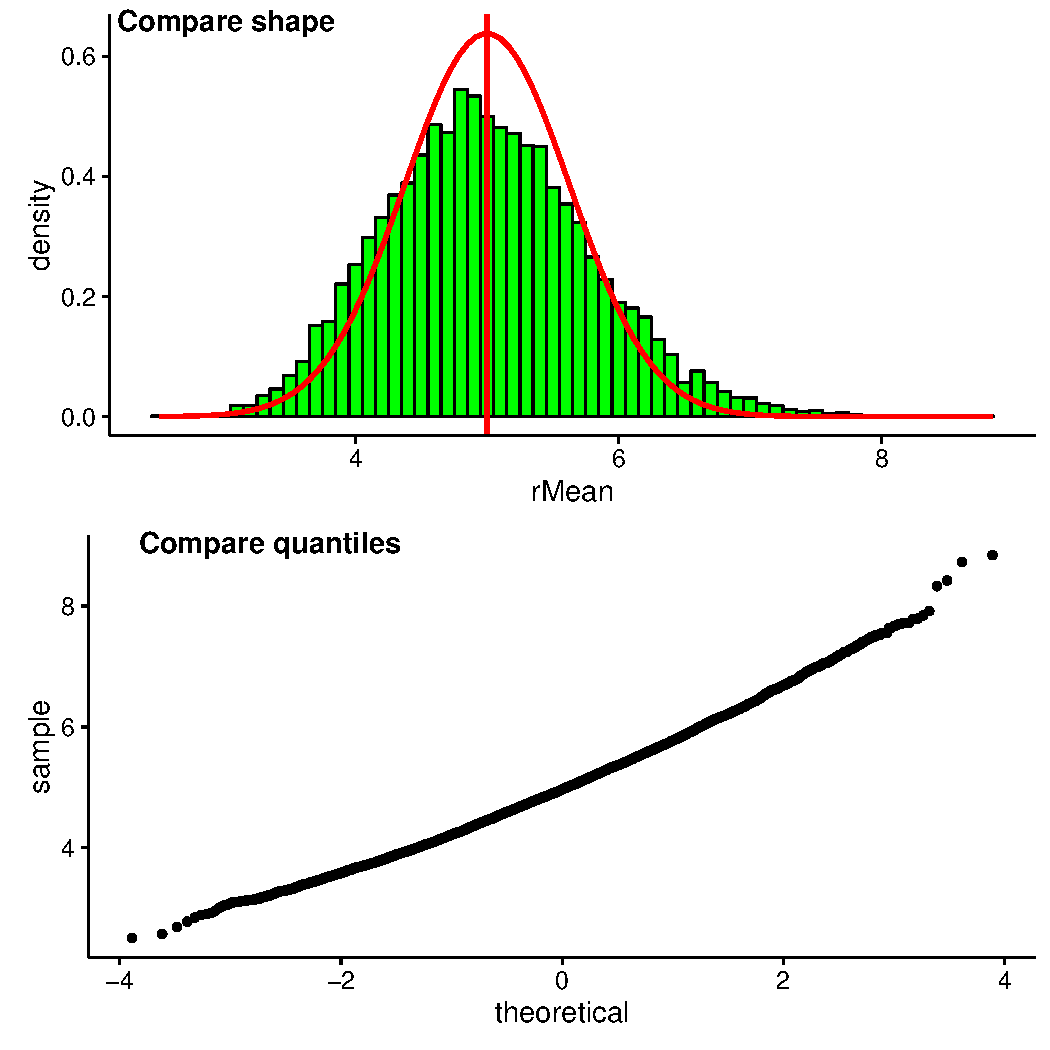
\includegraphics[width=\maxwidth]{figure/plots-1} 

\end{knitrout}
\section{Conclusion}

\fbox{
    \parbox[c][1.5\height]{\textwidth}{
        \textbf{As points are aligned in the qqnorm diagram and with the shape of the histogram, the distribution of the mean follows the normal distribution $\mathcal{N}$(5,0.625), as expected with the CLT.
    }}}
\end{document}
